\section{Methodology}

\subsection{Shots of the Orbiter grid}

% MISSING SHOT OF THE ENTIRE BLOCK

\begin{figure}[H]
 \centering
 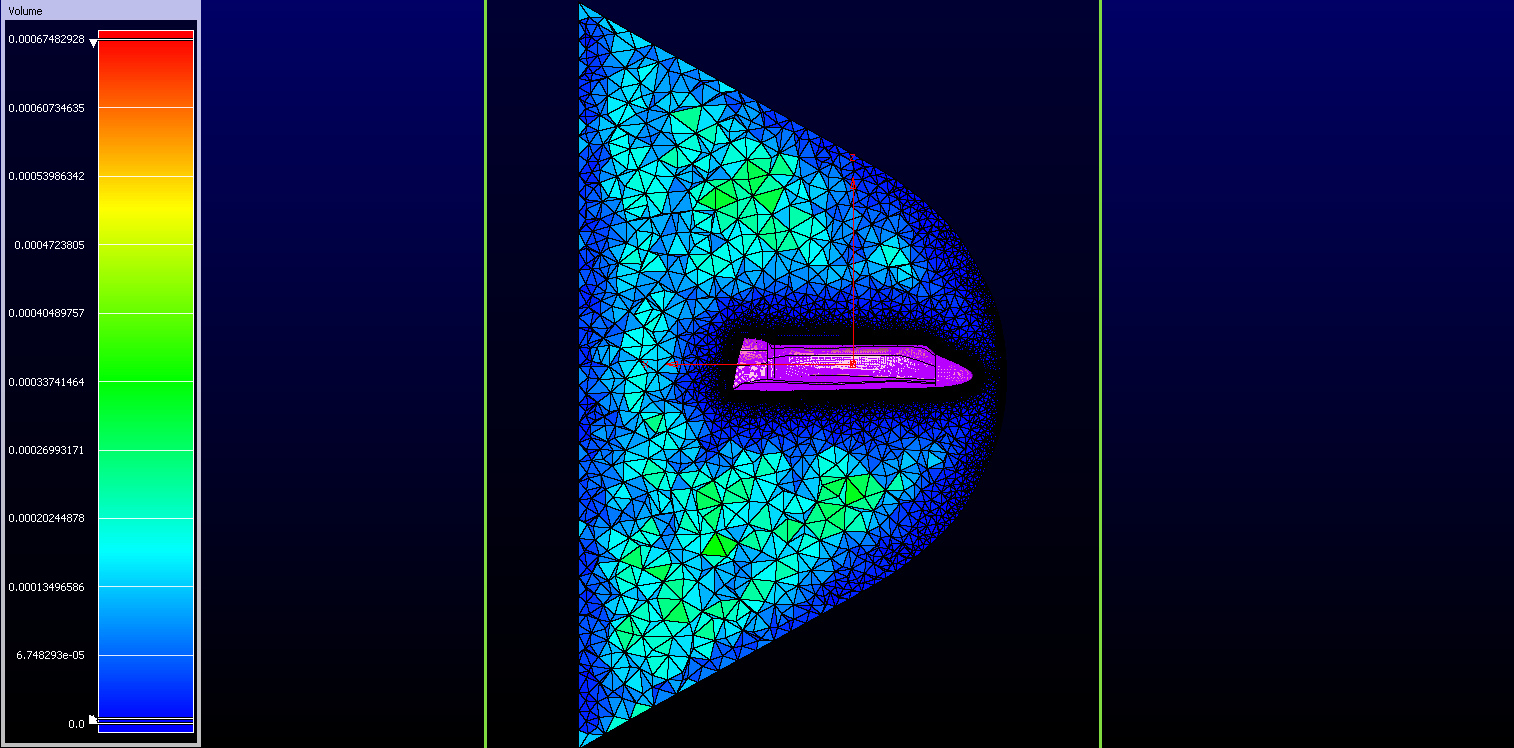
\includegraphics[width=\textwidth]{report_images/ss_entire_grid_trex_final.png}
 \caption{Entire grid of the orbiter}
 \label{fig: ss_entire_gred}
\end{figure}

\begin{figure}[H]
 \centering
 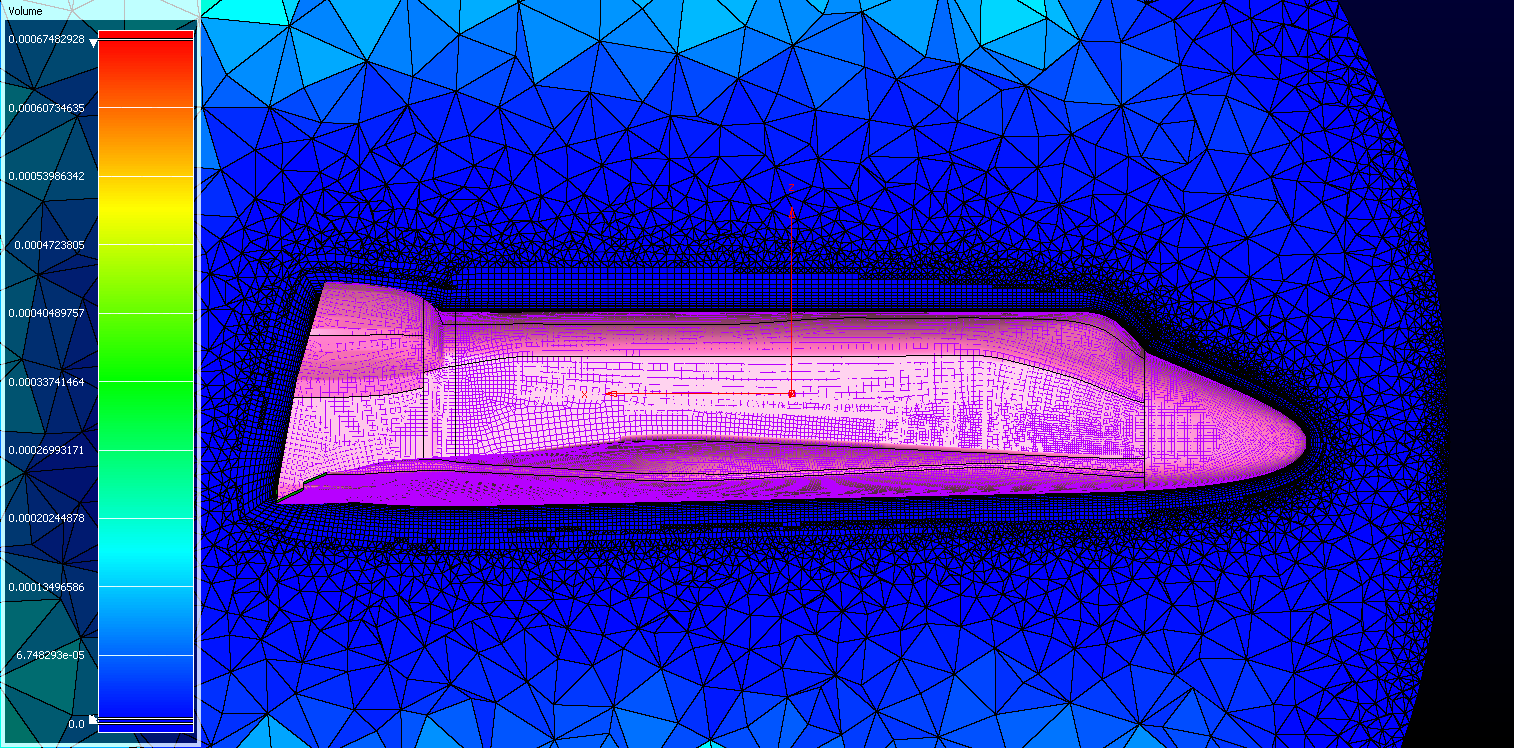
\includegraphics[width=\textwidth]{report_images/ss_surface_grid_trex_final.png}
 \caption{Surface grid of the orbiter}
 \label{fig: ss_surface_grid}
\end{figure}

\begin{figure}[H]
 \centering
 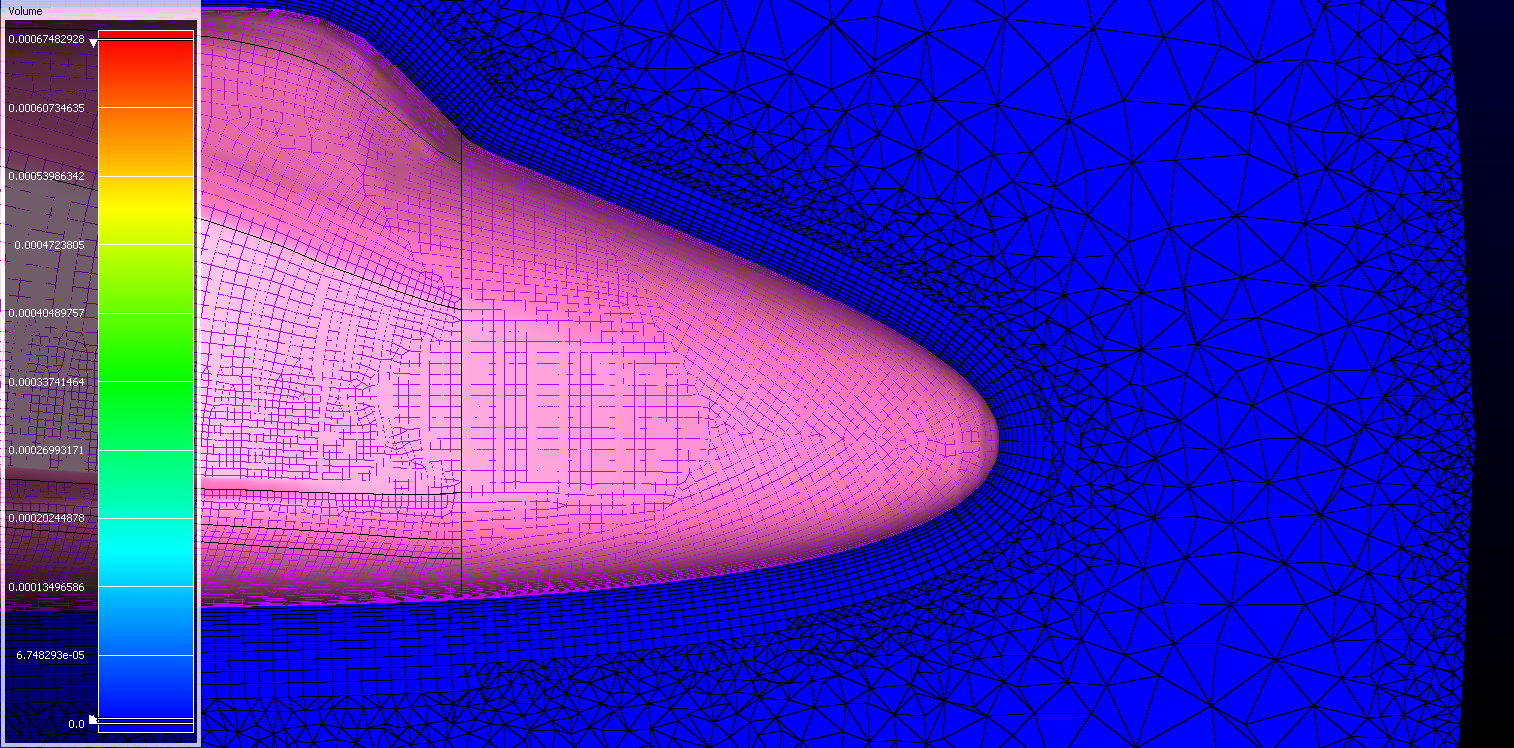
\includegraphics[width=\textwidth]{report_images/ss_nose_LE_trex_final.png}
 \caption{Nose of the orbiter}
 \label{fig: ss_nose_LE}
\end{figure}

\begin{figure}[H]
 \centering
 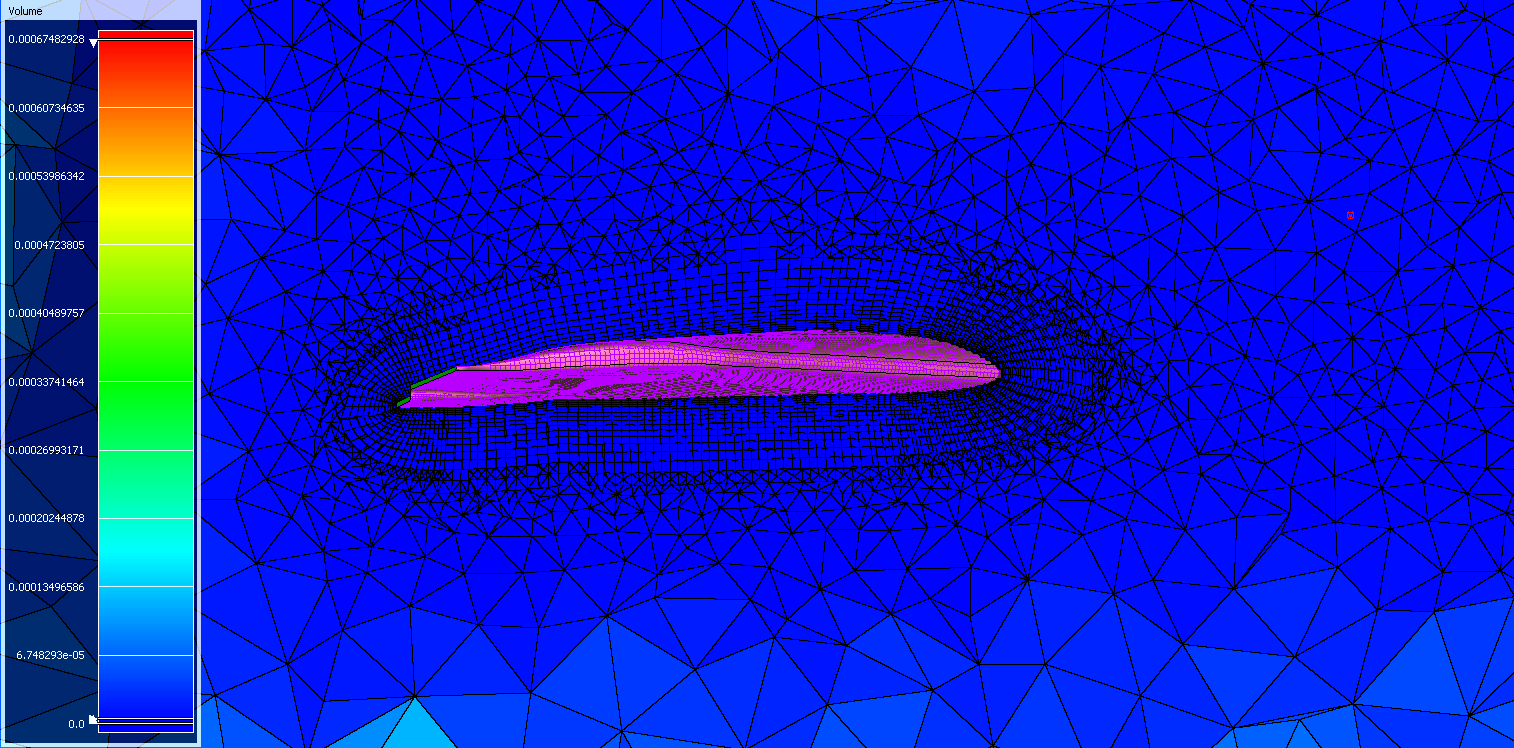
\includegraphics[width=\textwidth]{report_images/ss_wing_midspan_final.png}
 \caption{Midspan of the wing of the orbiter}
 \label{fig: ss_wing_LE}
\end{figure}


\subsection{Fluent setup}

%cell count: 1,375,480
%normal-to-wall spacing(s) used: 0.001
%min/max included angles: max: 179.844 deg min: 0.06222
%boundary conditions: symmetry: the symmetry plane; wall: orbiter surface; pressure far-field: inlet; pressure outlet: backwall.
%list reference values:
%area: 257.47 m^2 (projected in z) 1976 standard atmosphere calculator
%density: 0.0167207 (kg/m^3)
%enthalpy: 890742.9 (J/kg)
%length: 38.424 (m)
%pressure: 0 (gauage pressure)
%temperature: 227.13 K
%velocity: 1147.855 (m/s)
%viscosity: 1.789e-5 (kg/m/s)
%ratio of specific heats: 1.4
%
%list submodels chosen (i.e., viscous model selected), and provide numerical scheme and spatial accuracy used:
%
%implicit AUSM
%
%gradient: least squares cell based
%
%flow: first order upwind



\begin{table}[H]
\caption{General grid information}
	\centering
	\begin{tabular}{|l|p{4.5in}|} \hline
		Cell count & 1,375,480 Cells  \\ \hline
		Min/max included angles & \textbf{max}: 179.844 deg \textbf{min}: 0.06222 deg \\ \hline
		Normal-to-wall spacing & $\boldsymbol{\Delta}$\textbf{s} = 0.001 m \\ \hline
		Boundary conditions & \textbf{Inlet/hemispherical shell}: pressure far-field \newline \textbf{Outlet/back of hemispherical shell}: pressure outlet \newline \textbf{Orbiter surface (including backside)}: wall \newline \textbf{Plane of Symmetry}: symmetry \\ \hline
		Reference values & \textbf{Area}: 257.47 [m$^2$] \newline \textbf{Density}: 1.672e-02 [kg$\cdot$ m$^{-3}$] \newline \textbf{Enthalpy}: 8.907e+05 [J$\cdot$ kg$^{-3}$] \newline \textbf{Length}: 38.424 [m] \newline \textbf{Gauage pressure}: 0 [Pa] \newline \textbf{Temperature}: 227.13 [K] \newline \textbf{Velocity}: 1147.86 [m$\cdot$ s$^{-1}$] \newline \textbf{Viscosity}: 1.789e-05 [kg$\cdot$ m$^{-1}$s$^{-1}$] \newline \textbf{Ratio of specific heat}: 1.4 \\ \hline
		Submodels & \textbf{Density}: ideal-gas \newline \textbf{Specific heat}: piece-wise polynomial \newline \textbf{Thermal conductivity}: kinetic-theory \newline \textbf{Viscosity}: sutherland \\ \hline
		% THINK ABOUT A BETTER NAME FOR METHOD AND ACCURACY
		Numerical Scheme & Implicit AUSM \\ \hline
		Spatial Discretization & \textbf{Gradient}: least-squares cell based \newline \textbf{Flow}: first order upwind \\ \hline
	\end{tabular}
\end{table}